\chapter{Discussion}
%%%%%%%%%%%%%%%%%%%%%%%%%%%%%%%%%%%%%%%%%%%%%%%%%%%%%%%%%%%%%%%%%%%%%%%%%%%%%%%%%%%%%
%%%%%%%%%%%%%%%%%%%%%%%%%%%%%%%%%%%%%%%%%%%%%%%%%%%%%%%%%%%%%%%%%%%%%%%%%%%%%%%%%%%%%

In this chapter, the results presented in chapter four, including their limitations are discussed in relation to research and theories. In the beginning, the results of the case study will be discussed followed by the results of the survey.

To verify that the results of our survey are a good representative of the active programmers we decided to compare our results with the Stack Overflow’s 2018 developer survey results\footnote{\url{https://insights.stackoverflow.com/survey/2018/}}. Stack Overflow is a question and answer forum dedicated to computer programming and every year runs a survey among its users and shares it openly with the community. This year more than 100,000 developers participated in the survey, and its results were published shortly after our survey and could be considered as a good reference. 
Looking at the heat map of the location of the subjects, we see that there are similarities between the two surveys. Most of the respondents are from northern America, Europe, and India. Regarding gender, there were slightly more female participants in our study. There were almost double as much backend developers in Stack Overflow’s survey than ours. 

\citet{Stray2017a} also did a survey of distributed teams and found almost identical demographic results as our survey, which combined with the Stack Overflow results ensures us that our results are reliable. 
However, when it comes to time spent on active remote collaboration; there is a slight difference between our findings with \citet{Karis2016} who ran a survey among Google developers. Out of 501 responses they received, 6.6 percent stated that they were collaborating nearly all the time while in our case (n = 44), nobody was claiming to collaborate that much. Table \ref{table:collaboration} compares the results.
    
    
\begin{table}
\centering
\caption{Time spent on active remote collaboration} \label{table:collaboration}
\begin{tabular}{lcc}
\hline
\textbf{The frequency of active collaboration} & \textbf{Our results (n=44)} & \textbf{Google (n=501)} \\ \hline
None or nearly none of my time&11\%&10.8\%\\
Less than 1/4 of my time&64\%&53.1\%\\
Up to 1/2 of my time&20\%&22.8\%\\
More than half my time&5\%&6.8\%\\
Nearly all my time&0\%&6.6\%\\
&Total 100\%&Total 100\%\\
\hline
\end{tabular}
\end{table}

If we consider a typical workweek as forty hours, then this amount of remote collaboration counts as around 14\% of the whole people engaged in distributed teams spending at least 21 hours per week in active collaboration with distributed team members. Also, 24\% spend some time between 10 to 20 hours a week on remote collaboration. 

These numbers become even more meaningful if we look at the responses we have got about the challenges in the distributed work, where around half of the respondents have stated that time-zone differences and coordination are the biggest challenges in distributed work. 
If the task or the project that the team members are working on can be divided into parts that can partly be done and worked on individually and independent from other team members then it would be easier to collaborate remotely with other team members, since the time needed to work on a given task simultaneously is minimal or non-existent. 

The problem arises when two team members must work on the same task remotely; then it could be a huge challenge if the time difference is so much that at one place the sun is shining at the middle of the day while in the other part of the world it has past a few hours after midnight. 
Here there is a dilemma between having a development team that can work around the clock, 24 hours a day or a development team that are far less separated, both physically and by time. The choice might be dependent on kind of the project and tasks, but our research shows that there would be unexpected challenges in coordination and collaboration between team members that can affect the results gained by distributed team heavily. 

Finding of \citet{Ibrahim2015} also shows that temporal and geographical distance is the biggest challenge of distributed software development. More than 75 percent of the literature reported it as the number one challenge among the distributed teams. Distance differences also affect communication negatively in teams; it reduces the efficiency of communication between remote teams \citep{Dorairaj2011}.

\citet{Marlow2016} in their survey asked a question about the purpose of remote meetings. We did the same and Table \ref{table:remotepurpose} compares the results. According to the results of our survey, almost half of the respondents reported use scrum as their development method. So it is considered that the most stated reason for remote meetings is “status update.” “Information sharing” follows closely status update, while the status update is obviously about updating the whole team, information sharing might refer to meeting and collaboration with two team members.

\begin{table}
\centering
\caption{The purpose of remote meetings} \label{table:remotepurpose}
\begin{tabular}{lcc}
\hline
& \textbf{Our results} & \textbf{Marlow 2016} \\ \hline
Status update&27\%&33\%\\
Information sharing&21\%&18\%\\
Brainstorming&	15\%&	13\%\\
Conversation&	14\%&	12\%\\
Presentation&	12\%&	9\%\\
Other&	11\%&	14\%\\
\hline
\end{tabular}
\end{table}

Looking at the communication media used in distributed teams we see that just 17\% have stated that they use face-to-face meetings as a communication media, and later in another question when asked about the frequency of face-to-face meetings we see that 34\% of respondents have stated that they never meet face-to-face with other team members. This can be problematic and increases misunderstanding among the team \citep{Curtis1988}.\\



We discussed media synchronicity theory as an extension of media richness theory in Section \ref{sec:media}, and presented figure \ref{fig:maruping} which was an illustration of media synchronicity theory based on \citet{Maruping2004}. After going through the results of our survey and our case and examining Slack as a modern \ac{esn} we came to figure \ref{fig:mine} which reflects the changes that we have made to the \citeauthor{Maruping2004}'s (\citeyear{Maruping2004}) illustration. Here the white triangles shows the place of original image. Here videoconferencing gets a bit lower grade in "parallelism" because according to our experience and the survey results it falls behind face-to-face encounters and can not get much higher grade in that regard. When it comes to \ac{im} \citet{Maruping2004} have given a very low grade regarding symbol variety and parallelism, but fourteen years later we see that modern \ac{im}'s are quite rich in symbols and parallelism is easy to achieve. Another important point here is that Slack has also another feature which was not present in previous communication applications and that is the ability to edit the messages even after the message is sent. This "editability" feature is unique to modern \ac{esn}s such as Slack and can not be found in other ways of communication. In case of Slack, a user can edit his or her own posts without any time limitation and a small (edited) sign will be shown after the message so that the others will know that the message is changed (See figure \ref{fig:edit}).

\begin{figure}[!t]
\centering

\includegraphics[width=.6\textwidth]{edit.jpg}
\caption{An edited message in Slack}\label{fig:edit}
\index{figures}
\end{figure}

\begin{figure}[hbt!]
\centering
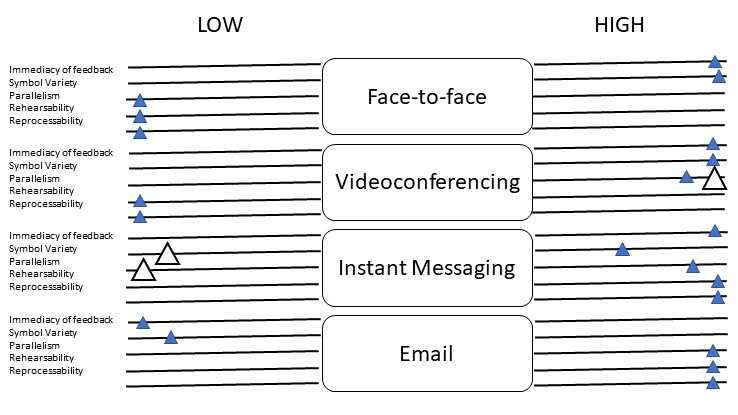
\includegraphics[width=.99\textwidth]{mine.jpg}
\caption{Media synchronicity theory, inspired by \citet{Maruping2004}}\label{fig:mine}
\index{figures}
\end{figure}


%%%%%%%%%%%%%%%%%%%%%%%%%%%%%%%%%%%%%%%%%%%%%%%%%%%%%%%%%%%%%%%%%%%%%%%%%%%%%%%%%%%%%
%%%%%%%%%%%%%%%%%%%%%%%%%%%%%%%%%%%%%%%%%%%%%%%%%%%%%%%%%%%%%%%%%%%%%%%%%%%%%%%%%%%%%
\chapter{Limitations}
%%%%%%%%%%%%%%%%%%%%%%%%%%%%%%%%%%%%%%%%%%%%%%%%%%%%%%%%%%%%%%%%%%%%%%%%%%%%%%%%%%%%%
%%%%%%%%%%%%%%%%%%%%%%%%%%%%%%%%%%%%%%%%%%%%%%%%%%%%%%%%%%%%%%%%%%%%%%%%%%%%%%%%%%%%%

Notwithstanding using a reliable research method, consisting of cutting the edge research and data collection and analysis schemes I am aware of the several limitations of my research. First, the lack of access to other means of communication used by team members in the case study, other than conversations in Slack channels. Other means of communication that could have been interesting to get access to were emails and private messages sent on Slack. The company was not able to retrieve private messages due to the type of Slack subscription they have which just allows for exporting of conversations in channels.

Second, due to the enormous amount of chat logs and the fact that all the logs needed to be coded manually, just a handful of chat logs from certain channels were coded. Although I tried to choose the channels that are common to other teams as well it would have been better to code more data from more Slack channels.

Third, the case study was limited just to one company and the findings might have been under the influence of the culture and other circumstances unique to that company. Also, the fact that the teams were located in the same time-zone and have somehow near European culture and background might also affect the results and make it harder to generalize.

And finally,  all the analysis is done just by one researcher, although that researcher is not biased. This can reduce the reliability of the research because the gathering of results and their interpretation is dependent on the knowledge and experience of the researcher. But I have tried to describe all the steps taken in detail so that the future researchers can follow the same steps and compare their results with mine.

%%%%%%%%%%%%%%%%%%%%%%%%%%%%%%%%%%%%%%%%%%%%%%%%%%%%%%%%%%%%%%%%%%%%%%%%%%%%%%%%%%%%%
%%%%%%%%%%%%%%%%%%%%%%%%%%%%%%%%%%%%%%%%%%%%%%%%%%%%%%%%%%%%%%%%%%%%%%%%%%%%%%%%%%%%%
\chapter{Conclusion and future work}
%%%%%%%%%%%%%%%%%%%%%%%%%%%%%%%%%%%%%%%%%%%%%%%%%%%%%%%%%%%%%%%%%%%%%%%%%%%%%%%%%%%%%
%%%%%%%%%%%%%%%%%%%%%%%%%%%%%%%%%%%%%%%%%%%%%%%%%%%%%%%%%%%%%%%%%%%%%%%%%%%%%%%%%%%%%